% Szablon, v. 3.9 p.wlaz@pollub.pl
% http://mat.pol.lublin.pl/~pwlaz/dyplom-latex

\documentclass[12pt, withmarginpar]{mwbk}
\include{_defs}
\begin{document}

\thispagestyle{empty}%brak numeracji


%%%%%%%%%%%%%%%%%%%%%%%%%%%%%%%%%%%%%%%%%%%%%%%%%%%%%%%%%%%%%%%
%%%%%tytuły definiuje jako makrodefinicje, gdyż zamierzam je%%%
%%%%%powtórzyć na stronie ze streszczeniami, to nic nie boli%%%
%%%%%a gwarantuje, że będą one takie same, i~tak ma być.%%%%%%%
%%%%%%%%%%%%%%%%%%%%%%%%%%%%%%%%%%%%%%%%%%%%%%%%%%%%%%%%%%%%%%%P.Wlaź
\newcommand\tytul{Dyfuzja wiedzy innowacyjnej w czasie i przestrzeni
                  na podstawie patentów z ostatnich dziesięciu lat}

\newcommand\tytulangielski{Diffusion of innovative knowledge 
                           in time and space based on patents 
                           from the last ten years}

\noindent
\hspace*{-3mm}\includegraphics[width=8.67cm]{logo.pdf}
\fontfamily{qhv}\fontsize{12pt}{15pt}\selectfont

\vfil 
\noindent Katedra Matematyki Stosowanej

\vfil\vfil\vfil\vfil


\fontsize{40pt}{50pt}\selectfont
\noindent Praca inżynierska

\fontsize{12pt}{15pt}\selectfont


\vfil
\noindent
na kierunku \emph{inżynieria i~analiza danych}
\vfil\vfil

\vspace{2cm}
\fontsize{16pt}{18pt}\selectfont
\noindent \tytul

\vspace{1cm}
\fontsize{16pt}{18pt}\selectfont
\noindent \tytulangielski

\vfil\vfil\vfil\vfil
\fontsize{16pt}{20pt}\selectfont

\noindent 
Adam Jakubczak

\vfil
\fontsize{12pt}{15pt}\selectfont
\noindent
numer albumu: 098750


\vfil

\noindent
promotor: dr inż. Korneliusz Pylak

\vfil\vfil\vfil

\fontsize{9pt}{12pt}\selectfont

\noindent
Lublin 2025

\normalsize \rm

\tableofcontents

\chapter*{Wstęp}

Dyfuzja wiedzy innowacyjnej w czasie i przestrzeni to proces
rozprzestrzeniania się nowych technologii pomiędzy podmiotami
w lokalnym otoczeniu.

Wiedza innowacyjna jest kluczowym elementem rozwoju gospodarczego.
To jej przypisuje się siłę napędową dla wzrostu gospodarczego
w nowoczesnych gospodarkach. Zrozumienie procesów dyfuzji 
wiedzy innowacyjnej może pozwolić na budowanie lepszych 
warunków dla rozwoju gospodarczego.

Patenty są dobrym wskaźnikiem tego zjawiska z 2 powodów:
po pierwsze dotyczą wyłacznie innowacji --- takie jest ich zadanie,
po drugie zawierają informacje na temat ich twórców, co pozwala
na stwierdzenie o ich lokalizacji, która jest kluczowym elementem
w procesie dyfuzji wiedzy.

\todonote{wstęp do poprawy na koniec}

\chapter{Przegląd literatury}\label{ch:intro}

\section{Wprowadzenie do tematu dyfuzji wiedzy}

Dyfuzja wiedzy innowacyjnej jest przedmiotem zainteresowania
wielu badaczy. Przegląd dzieł związanych z tematem od różnych
autorów pozwala na zrozumienie tego jakie są kluczowe elementy
procesu dyfuzji wiedzy innowacyjnej i czym właściwie ona jest.

Nonaka \cite{No-98} rozdziela informację od wiedzy na podstawie
tego jak została zaadaptowana przez podmioty i w jakim
kontekście jest umieszczona. Pogląd rozdziału informacji
od wiedzy powielają także Morone i Taylor \cite{Mo-Ta-09}.

Nonaka \cite{No-98} rozdziela także wiedzę na jawna i ukrytą.
Pathirage \cite{Pa-08} wskazuje, że taki rozdział jest dominujący 
w literaturze przedmiotu. Alwis i Harmann \cite{Al-Ha-08} dają dobry 
wgląd w to czym jest wiedza ukryta poprzez zagłębienie się 
w literaturę. Wskazują, że wiedza ukryta jest kluczowym 
elementem innowacyjności firm i jest ściśle powiązana z 
procesem dyfuzji wiedzy innowacyjnej.

Częstym cytatem w literaturze przedmiotu jest stwierdzenie
Michaela Polanyiego: \textit{Wiemy więcej niż potrafimy powiedzieć},
gdzie z faktu, że \textit{wiemy więcej} wnioskujemy o istnieniu czegoś
ponad to czym jest wiedza jawna - tego \textit{co potrafimy powiedzieć}.

Dużą rolę w zachowaniu konkurencyjności firm przypisuje się
zarządzaniu wiedzą, a szczególnie wiedzą ukrytą \cite{No-98}.
Nonaka, jak inni \cite{Mo-16}, \cite{Ga-Th-14}, definiuje wiedzę ukrytą
jako zaprzeczenie wiedzy jawnej. Wiedza jawna to taka
przechowywana na wszelkich nośnikach, ale też możliwa w artykulacji
do innych osób. Wiedza ukryta, jako jej przeciwieństwo,
jest trudna albo niemożliwa do wyrażenia słowami albo symbolami.
Jest nabywana podczas praktyki albo obserwacji \cite{No-98}.

Nonaka \cite{No-98} definiuje model procesu tworzenia wiedzy w firmie, 
jako 4-etapową spiralę, w której kolejne kroki to: nabywanie wiedzy
ukrytej, jej synteza w wiedzę jawną, standaryzacja wiedzy jawnej
i adaptacja wiedzy jawnej przez pracowników do wiedzy ukrytej.
Podobny pogląd na powstawanie wiedzy przedstawiaja Morone i 
Taylor \cite{Mo-Ta-09} stwierdzając, że wiedza zawsze jest początkowo
wiedzą ukrytą, a dopiero w procesie jej artykulacji staje się
wiedzą jawną.

Istotą przepływu wiedzy ukrytej jest to jakie warunki panują
w firmie. Nonaka \cite{No-98} wskazuje jako modelowe, firmy japońskie, w
których panuje redundancja informacji, co sprawia, że pracownicy
posiadają podobny zestaw wiedzy ukrytej. Alwis i Hartmann \cite{Al-Ha-08}
także przypisują jakość dyfuzji wiedzy ukrytej do organizacji
firm twierdząc, że likwidacja barier wewnętrznych w firmie jest
kluczowa dla efektywnego przepływu wiedzy.

Bathelt i Feldman \cite{Ba-Fe-11} także rozważają powstawanie wiedzy
innowacyjnej jako proces przerabiania aktualnej wiedzy na nową.
W nieścisły sposób łączy się to z modelem Nonaka \cite{No-98}, gdzie
wiedza także ulega ciągłej transformacji. 

Dalej \cite{Ba-Fe-11}, na podstawie literatury, 
stwierdzają o ograniczeniach przestrzennych jakie wiążą się z
rozprzestrzenianiem się wiedzy. Wynikają one między innymi z
przywiązaniem ludzi do ich miejsca zamieszkania, czy ulokowaniem
środków firm, czy całego sektora w jednym regionie.

Samo rozprzestrzenianie się wiedzy można podzielić na 2 typy:
dyfuzję i wymianę \cite{Mo-Ta-09}. Wymiana polega na
przepływnie wiedzy między podmiotami na podstawie uzgodnionych
oraz świadomych działań w trakcie których następuje symbiotyczna
interakcja, w której jedna strona zyskuje wiedzę, a druga
wiedzę inną albo korzyści niezwiązane z samą wiedzą. W kontrze
do wymiany, dyfuzja to proces nieświadomego przepływu samej wiedzy.
Morone i Taylor wskazują, że w procesie dyfuzji, podmioty będące
odbiorcami mogą wykorzystywać mimowolne przepływy wiedzy na
swoją korzyść. Dalej zastrzegają, że takiemu procesowi dyfuzji
podlega wiedza ukryta, a jej przyswojenie wymaga zdolności 
(pojemności) absorpcyjnych (ang. \textit{absortive capacity}).

Taylor i Morone \cite{Mo-Ta-09} rozkładają dyfuzję na 3 procesy:
rozlewanie \foreign{ang}{spillover}, transfer oraz integrację. Rozlewanie
i transfer to procesy podobne z tą różnicą, że transfer jest
określony jako przepływ z pierwotną intencją jego zaistnienia.
Oba te procesy wymagają istniejącej wcześniej wiedzy, która
umożliwia absorbcję nowej wiedzy. Integracja z kolei to proces,
w który istniejąca wiedza jest aplikowana w innym kontekście.

Klarl \cite{Kl-14} twierdzi, że dyfuzja wiedzy to proces społeczny,
który napędzają, po pierwsze: więzi między ludźmi i grupami,
a po drugie cechy indywidualne ludzi. To jak silne są więzi
w grupie oraz między grupami ma znaczący wpływ na szybkość
rozprzestrzeniania się wiedzy. Klarl twierdzi, że można
wyróżnić w populacji grupy o różnych miarach dyfuzji wewnątrz,
jak i po między grupami oraz z zewnątrz. Dodatkowo zakłada
ograniczenia przestrzenne związane z dyfuzją wiedzy - sieć
jest tym słabsza im bardziej jest rozproszona w przestrzeni.

Boone, Ganeshan, i Hicks \cite{Bo-Ga-Hi-08} przedstawiają znane już zjawisko
starzenia się wiedzy jako proces, w którym wiedza nagromadzona
w organizacji przekłada się na coraz mniejszą wartość dla firmy.
Mimo, że innowacje są efektem nadbudowywania wiedzy to należy
się domyślić, że jej starzenie skutecznie temu zapobiega. 
Zaznaczają też, że szybkość starzenia zależy od branży, ale też
działań jakie są podejmowane aby mu zapobiegać.

Z podobną tezą występują Grubler i Nemet \cite{Gr-Ne-13}, określając
zjawisko starzenia się jako \textit{oduczanie} - przeciwieństwo nauki.
Podają ku temu 2 przyczyny: zanikanie wiedzy związane z rotacją
pracowników oraz zanikanie wiedzy związane z innowacjami, które
następują na tyle szybko, że nie sposób dostosować do nich starej
wiedzy. Zanikanie związane z rotacją wiąże się z tym, że
przeniesienie, czy zwolnienie pracownika sprawia, że ten,
posiadający wiedzę ukrytą, nie używa jej już w organizacji.
Grubler i Nemet zaznaczają, że to właśnie wiedza ukryta jest
szczególnie wrażliwa na starzenie.

Frenken, Van Ooor i Verburg \cite{Fr-Oo-Ve-07} opisują pojęcie pokrewnej i
niepokrewnej różnorodności wiedzy. Różnorodność pokrewna dotyczy
wiedzy z jednej dziedziny, a niepokrewna z różnych dziedzin.
Badacze wskazują, że różnorodność pokrewna sprzyja bardziej
dyfuzji wiedzy niż różnorodność niepokrewna.



\section{Patenty w literaturze przedmiotu}

Patenty są istotnym wskaźnikiem dyfuzji wiedzy innowacyjnej
między środowiskami akademickimi, a rynkiem \cite{Lo-Br-08}.
Dają one informacje o tym jak wiedza zdobywana na uczelniach
przenika do firm i jak jest wykorzystywana w praktyce.

Sorenson i Fleming \cite{So-Fl-04} wskazują w swojej pracy na związek
między cytowaniami w patentach, a tym jak te same patenty są
cytowane. W badaniu wykazali, że patenty, które cytują częściej
są także częściej cytowane. Wynika z tego, że przepływ wiedzy
jest przyśpieszany przez uwzględnienie wiedzy jaka została
już wcześniej zgromadzona.

Acs, Anselin i Varga \cite{Ac-An-Va-02} określają związek między patentami,
a innowacjami jako zależność nieidealną, gorszą od literatury
badawczej ale porównywalną z nią. Wskazują na zaletę jaką może
być uwzględnienie przez patenty innowacji z mniejszych organizacji,
co często jest pomijane w opracowaniach naukowych.

Verspagen i Schoenmakers \cite{Ve-Sc-00} podają 2 powody, dla których
patenty mogą być solidnym wyznacznikiem dyfuzji w ekonomii:
w kontekście dużych firm zakładają istnienie zespołów R\&D do
analizy patentów na rynku, a co za tym idzie nabywania wiedzy
o nich. Drugi powód to cytowania patentowe, które wskazują
na związki między wynalazcami - duże podobieństwo jest miarą
tego jak wiedza ulega dyfuzji na tym wymiarze.


\section{Podsumowanie}

Na podstawie wcześniejszego przeglądu literatury można wyprowdzić
pewne ogólne definicje, co do których będą stawiane tezy.

Jednym z podstawowych założeń jest rozdział wiedzy od samej informacji.
Logicznie można też stwierdzić, że wiedza jest podzbiorem informacji,
która wyróżnia się tym, że jest interpretowana przez człowieka w danym
kontekście.

\Needspace{5\baselineskip}
\begin{defi}
Informacja ($I$) --- ogólny termin odnoszący się do wszelkich form wiedzy, 
umiejętności, doświadczeń, przekonań przechowywanych na różnych nośnikach 
albo w ludzkiej pamięci - świadomie lub nieświadomie.
\end{defi}

\begin{defi}
Wiedza ($W$) --- informacja zinterpretowana przez człowieka w danym kontekście.
\begin{center}
\begin{math}
W \subset I
\end{math}
\end{center}
\end{defi}

To czym jest informacja można odnieść zarówno do danych
przechowywanych na serwerach, tez zawartych w dziełach naukowych,
jak i umiejętności praktycznych wszelkiego rodzaju, np.
balans ciałem podczas jazdy na rowerze. W odróżnieniu od informacji, 
wiedza jest zawsze związana z jakimś kontekstem oraz tym 
jak jest ona interpretowana przez daną jednostkę.

\Needspace{5\baselineskip}
\begin{defi}
Wiedza jawna ($W_j$) \foreign{ang}{explicit knowledge} --- wiedza
zapisywana na nośnikach informacji i przekazywana za pomocą
języka, symboli, obrazów, dźwięków.
\end{defi}

Wiedza jawna jest ogólnie dostępna z samej jej definicji - przekazywana
w słowach ulega upowszechnieniu w postaci rozmów i wszelkich mediów: 
książek, artykułów, prezentacji, filmów, itp. 

\Needspace{5\baselineskip}
\begin{defi}
Wiedza ukryta $W_u$ --- przeciwieństwo wiedzy jawnej:
wiedza, której nie da się uchwyciś słowami czy symbolami,
nabywana podczas praktyki.
\begin{center}
\begin{math}
W_u = W \setminus W_j
\end{math}
\end{center}
\end{defi}

W anglosaskiej literaturze określana jest jako \textit{tacit knowledge}.
Nazwa pochodzi od łacińskiego \textit{tacitus} - \textit{milczący}.
Dobrze oddaje naturę tej wiedzy, bo oprócz tego, że jest ona
trudna do uchwycenia, to jej specyfika wynika właśnie z niemożności
do jej artykulacji w języku. Jej specyfikę podsumowuje popularne 
w literaturze stwierdzenie \textit{Wiemy więcej niż potrafimy powiedzieć}, 
Michael Polanyi.

\Needspace{5\baselineskip}
\begin{defi}
Wiedza innowacyjna $W_i$ --- wiedza rozszerzająca dotychczasową
wiedzę, która prowadzi do rozwiązania aktualnych problemów.
\begin{center}
\begin{math}
W_i \subset W\qquad
W + W_i = W' \supset W
\end{math}
\end{center}
\end{defi}

Wiedza innowacyjna jest zawsze w jakimś stopniu nowa, ale
niekoniecznie musi być to coś zupełnie nowego. Może to być
również modyfikacja istniejącej wiedzy i najczęściej tak
właśnie powstaje - poprzez nadbudowywanie na istniejącej wiedzy.

\begin{defi}
Dyfuzja wiedzy innowacyjnej --- proces czasowy przepływu 
wiedzy innowacyjnej między podmiotami, występujący szczególnie
w lokalnej przestrzeni.
\end{defi}

Jest to \textbf{mimowolna} transmisja wiedzy w czasie i przestrzeni,
która wiąże się z przepływem wiedzy z ośrodków o dużej
koncentracji do sąsiadujących z nim podmiotów o mniejszej
koncentracji wiedzy.

Kluczowa w dyfuzji wiedzy innowacyjnej jest wymiana wiedzy
twarzą w twarz. Wielu autorów podkreśla, że wiedza ukryta,
która jest kluczowym elementem innowacyjności. Nie ulega
ona transmisji poprzez media, ponieważ jest ona niewerbalna.
W konsekwencji do jej rozprzestrzeniania potrzebne są spotkania
i interakcje między ludźmi podczas jej praktyki. Publikacje
naukowe zwracają też uwagę na istotę zaangażowania w rozszerzaniu
się tego rodzaju wiedzy, które jest łatwiej zainicjować w
sytuacjach socjalnych niż rozgrywających się na polu wirtualnym,
czy w postaci innych środków komunikacji.

Ograniczenia występowania tego rodzaju sytuacji są dość oczywiste i
wynikają między innymi z przestrzeni w jakiej operują ludzie.
Zazwyczaj są to ograniczenia do przestrzeni lokalnej, co sprawia,
że dyfuzja wiedzy innowacyjnej jest ograniczona do pewnego obszaru.
Nawet w lokalnych warunkach mogą dochodzdić dodatkowe obciążenia
takie jak bariery fizyczne, kulturowe czy wynikające z hierarchii
organizacyjnej albo struktury społecznej.


\Needspace{15\baselineskip}
\subsection{Patent jako narzędzie ochrony wiedzy innowacyjnej}

\begin{defi}
\textbf{Patent} --- forma ochrony prawnej udzielana na nieużywane, 
albo nieopatentowane wcześniej wynalazki, które wykazują 
zastosowanie w przemyśle. Powinny też być nieoczywiste dla 
ekspertów dziedzinowych.
\end{defi}

W Polsce przydzielaniem i ochroną patentów zajmuje się \ac{UPRP}, 
na poziomie europejskim jest to \ac{EPO}, a światowa organizacja 
to \ac{WIPO}.

Wartość patentów jako wskaźników dyfuzji wiedzy innowacyjnej
wynika z charakterystyki patentów jako narzędzi ochrony wiedzy.
Z definicji prawnej, patenty muszą reprezentować wiedzę innowacyjną
i być nowe, nieoczywiste oraz nadające się do praktycznego
zastosowania. Z tego właśnie powodu można przypuszczać, że
w pewnym stopniu oddają one stan faktyczny w dziedzinie innowacji.
Kolejnym atutem patentów jest ich klasyfikacja.
Patenty są klasyfikowane według międzynarodowej klasyfikacji
patentowej \ac{IPC}, dzięki czemu analizować je pod kątem dziedzinowym.
Dane dotyczące patentów są dostępne publicznie, co daje 
szerokie możliwości do ich analizowania oraz publikowania efektów
prac. Ponadto każdy patent jest przypisany do właściciela, oraz
na potrzeby formalne zawiera informacje o autorach, co pozwala
na budowanie sieci współpracy między podmiotami.

Mimo tych zalet, patenty mają swoje ograniczenia. Przede wszystkim
nie wszystkie wynalazki są opatentowane. Te opatentowane z kolei
mogą nie być wykorzystywane w praktyce, co sprawia, że nie
wszystkie innowacje są reprezentowane w danych patentowych.
Ponadto, patenty są zazwyczaj zgłaszane przez duże firmy, co
może prowadzić do zniekształcenia obrazu innowacyjności w
danej dziedzinie.

\begin{acronym}
  \acro{UPRP}{Urząd Patentowy Rzeczypospolitej Polskiej}
  \acro{EPO}{European Patent Office}
  \acro{WIPO}{World Intellectual Property Organization}
  \acro{MKP}{Międzynarodowa Klasyfikacja Patentów}
  \acro{IPC}{International Patent Classification}
  \acro{API}{Application Programming Interface}
  \acro{URI}{Uniform Resource Identifier}
  \acro{URL}{Uniform Resource Locator}
  \acro{OCR}{Optical Character Recognition}
  \acro{XML}{Extensible Markup Language}
\end{acronym}

\chapter{Źródła danych patentowych}\label{ch:data}

\include{src}

\section{Dane patentowe}

W danych ze zbioru \ac{UPRP} można wyróżnić kilka kategorii informacji
związanych z badanym tematem. Są to daty związane z procesem urzędowym
patentu, klasyfikacje patentowe, dane przestrzenne oraz dane osobowe
osób związanych z patentami.

\subsection{Dane przestrzenne}

Dane przestrzenne odnoszą się do miejsc z jakimi są powiązane
osoby albo organizacje związane z patentami. Pozostawia to więc 
różne możliwości analizy przestrzennej:

\begin{enumerate}
\item[$A$:] przypisanie każdego patentu do pojedynczej lokalizacji;
\item[$B$:] przypisanie patentu do wielu lokalizacji.
\end{enumerate}

W przypadku $A$ powstaje problem przypisania głównej lokalizacji.
Jest to kwestia $A_1$ priorytetowania organizacji ponad osoby, bądź
odwrotnie, oraz $A_2$ wyboru głównej osoby/organizacji.
Problem $A_1$ wiąże się z potencjalnymi różnicami w modelu zależnie
od wybranego podejścia. Problem $A_2$ może być niejednoznaczny
w rozwiązaniu z powodu zbyt małego zakresu informacji zawartych w danych.
Wymagałoby to dodatkowych danych z samego procesu powstawania wynalazku,
co jest poza zakresem tej pracy.

Dalsza analiza odnosi się wyłącznie do podejścia $B$.
Patent może mieć więc kilka lokalizacji, żadna nie jest określona jako główna.

Problemem jest także to, że dane zawierają wyłącznie nazwy miast, 
więc ich umieszczenie na mapie wiąże się z wadami: 
nazwy nie są unikalne --- w takim przypadku używany jest algorytm minimalizacji 
odległości, tak żeby wybrać optymalną kombinację. 
Wynika z tego oczywiste obicążenie. 
Po za tym nazwy mniejszych miejscowości mogą być duplikatami
nazw miast. Pewne powiązanie jest w takim przypadku niemożliwe
w wykonalny sposób na podstawie patentowych informacji.
Co za tym idzie rozważane są wyłącznie lokacje uważane za polskie miasta.
\todonote{przypis}

Mimo powyższych uproszczeń braki danych ciągle są obecne. Ich uzupełnianie
jest opisane w dalszej części pracy. Poniżej znajdują się 2 wykresy. 
Pierwszy przedstawiaja ilość danych dotyczących osób, dla których 
umieszczono informacje o lokalizacji. Widać w nim datę graniczną początkową,
która świadczy o momencie rozpoczęcia rejestrowania danych lokalizacyjnych.
Interesujący jest również spadek w roku 2004. Należy przypuszczać, że wynika
on ze zmiany metodologii zbierania danych osobowych po przystąpieniu
Polski do Unii Europejskiej.
Dla lat 2013-2022, czyli okresu zainteresowania analizy,
widać względną stabilność ilości danych z widocznym
spadkiem ich przyrostu rocznego. 



\halffigdraft{../fig.png}
{ Stan uzupełnienia informacji
  o geolokalizacjach,
  w Polsce,
  osób i organizacji 
  pełniących role patentowe 
  w aplikacjach patentowych}


\newpage
\begin{multicols}{2}

Opis tego jak uzupełnione są braki danych znajduje się w kolejnej sekcji.
Obok znajduje się wykres ilustrujący ilość patentów z geolokalizacjiami,
zgodnie z tym jak zostały określone.

\halffig{../fig/F-geoloc-eval.subj.png}
{ Stan uzupełnienia informacji o geolokalizacjach, w Polsce, 
  osób i organizacji  pełniących role patentowe
  w aplikacjach patentowych}

\end{multicols}

\newpage
\begin{multicols}{2}

\halffig{../fig/map.subj.png}
{Mapa rozrzutu geolokalizacji osób pełniących role patentowe}

\halffig{../fig/map-meandist100.subj.png}
{Mapa średniej odległości do innych osób pełniących role patentowe do 100 km}

\columnbreak

\halffig{../fig/map-meandist.subj.png}
{Mapa średniej odległości do innych osób pełniących role patentowe}

\halffig{../fig/map-meandist50.subj.png}
{Mapa średniej odległości do innych osób pełniących role patentowe do 50 km}

\end{multicols}

\begin{multicols}{2}

\halftable{../fig/T-meandist.subj.png}{Statystyki dotyczące średnich odległości}

\begin{uwaga}
Średnia odległość po między geolokalizacjami patentowymi jest ważona ---
ilość patentów pochodzących z danej geolokalizacji jest wagą tego punktu.
\end{uwaga}

\end{multicols}

Obszary peryferyjne to miejsca odległe od centrów, w tym przypadku
głównych źródeł aplikacji patentowych. Wyznaczamy je poprzez obliczenie
średniego dystansu do innych osób pełniących role patentowe.
Oprócz dystansu do każdego innego punktu, warto jest ograniczyć
tę statystykę do pewnego obszaru. Jak wcześniej zaznaczono, Polska
nie jest jednorodna przestrzennie pod tym względem, stąd peryferyjność
nie może być rozumiana tylko na krajowym poziomie, ale również lokalnym.

Rysunek \ref{../fig/map-meandist.subj.png} przedstawia średni dystans
do innych osób pełniących role patentowe w Polsce. Widać, że Warszawa
jest najbardziej centralnym punktem, co jest zgodne z wcześniejszymi
obserwacjami. To samo dotyczy okręgu Katowic. Na podstawie tej statystyki 
należy przypuszczać, że są to regiony o względnej bliskości 
do innych źródeł patentowych na poziomie krajowym.

Na rysunkach \ref{../fig/map-meandist100.subj.png} oraz
\ref{../fig/map-meandist50.subj.png} przedstawiono ten sam
wskaźnik, ale ograniczony do obszaru o promieniu odpowiednio 100 i 50 kilometrów.
\todonote{potrz. wyjaśn.}



\subsection{Rejestr dat związanych z patentami}

Poszczególne czynności związane z ochroną patentów są rejestrowane.
Każde wydarzenie jest powiązane z konkretną datą kalendarzową.
Można wyróżnić kilka typów wydarzeń związanych z patentami:

\begin{multicols}{2}

\begin{itemize}
\item publiczne ujawnienie \foreign{ang}{exhibition}
\item roszczenia z pierwszeństwa \foreign{ang}{priority claim} --- 
      data rozszczenia sprzed rozpoczęcia procesu patentowania dla wybranego urzędu
\item regionalna deklaracja \foreign{ang}{regional filing}\todonote{potrz. wyjaśniene}
\item deklaracja \foreign{ang}{filing}\todonote{potrz. wyjaśniene}
\item aplikacja \foreign{ang}{application} --- data złożenia aplikacji
\item przyznanie ochrony \foreign{ang}{grant}
\item decyzja urzędowa
\item publikacja
\end{itemize}
\todonote{potrz. źródło}

\columnbreak
\halffig{../fig/event.UPRP.png}
{Wydarzenia związane z patentami w kolejnych latach}

\end{multicols}

Powyższy wykres (\ref{../fig/event.UPRP.png}) obrazuje kolejne lata i to jakie
działania podejmował urząd w stosunku do składanych patentów. Urząd funkcjonuje
ponad 100 lat\todonote{od którego roku lepiej nap.} i widać to także na wykresie.
Widać na nim historyczne zdarzenia takie jak 2 Wojna Światowa (spadek w latach 39-45) 
oraz upadek ustroju komunistycznego w Polsce w latach (nagłwy wzrost 89-90) oraz
przystąpienie Polski do Unii Europejskiej (spadek w 2004).
Zmiany ustrojowe wiążą się także ze zmianem rozkładu rejestrowanych wydarzeń.
Przed latami 90 rejestrowane były wyłącznie daty aplikacji i grantów.
Następnie zaczęto rejestrować także inne, wcześniej wymienione, 
wydarzenia związane z patentami.

\newpage
\begin{multicols}{2}

Zmienność danych geolokalizacyjnych jest niewidoczna w ciągu badanego okresu, co obrazuje
wykres obok. W latach 2013-2022 nie widać znaczących zmian w rozrzucie źródeł
aplikacji patentowych.

\columnbreak
\halffig{../fig/map-13-22.subj.png}{
  Mapa rozrzutu geolokalizacji osób
  pełniących role patentowe
  w różnych okresach czasu
}

\end{multicols}



\newpage
\subsection{Klasyfikacje patentów}

Klasyfikacje patentowe to systemy, które pozwalają na przypisanie
patentów do odpowiednich dziedzin.

\subsubsection{Międzynarodowa Klasyfikacja Patentów}

W Polsce funkcjonuje klasyfikacja
\ac{MKP}, czyli \ac{IPC}. Zapis klasyfikacji w tym systemie to ciąg
cyfrowo-literowy składający się z 4 części:

\begin{enumerate}
    \item Dział - najwyższa hierarchia złożona z 8 kategorii
    \begin{itemize}
        \item ma tytuł informacyjny
        \item każdy tytuł działu ma swój symbol: A, B, C, D, E, F, G albo H
        \begin{itemize}
            \item A – podstawowe potrzeby ludzkie
            \item B – różne procesy przemysłowe; transport
            \item C – chemia; metalurgia
            \item D – włókiennictwo; papiernictwo
            \item E – budownictwo; górnictwo
            \item F – budowa maszyn; oświetlenie; ogrzewanie; uzbrojenie; technika minerska
            \item G – fizyka
            \item H – elektrotechnika
        \end{itemize}
        \item poddział - każdy dział może zawierać poddział, który nie jest oznaczany symbolem
    \end{itemize}
    \item Klasa - drugi poziom hierarchii
    \begin{itemize}
        \item ma tytuł informacyjny
        \item oznaczana przez liczbę 2-cyfrową
        \item zakres klasy - skrótowa informacja o treści klasy
    \end{itemize}
    \item Podklasa - trzeci poziom hierarchii
    \begin{itemize}
        \item ma tytuł informacyjny
        \item oznaczana dużą literą
        \item ma zakres i tytuł pomocniczy
    \end{itemize}
    \item Grupa - czwarty poziom hierarchii
    \begin{itemize}
        \item 2 zestawy cyfr oddzielone ukośnikiem
        \begin{itemize}
            \item zestaw pierwszy składa się od 1 do 3 cyfr i określa grupę główną
            \item zestaw drugi składa się z 2 cyfr i określa grupę pomocniczą, grupa główna jest oznaczana 00
        \end{itemize}
        \item grupa ma tytuł informacyjny, podgrupa ma bardziej szczegółowe hasło
    \end{itemize}
\end{enumerate}



\subsubsection{Wspólna Klasyfikacja Patentów}

\ac{CPC} to klasyfikacja stworzona przez \ac{EPO} i \ac{USPTO}
jako wspólny wysiłek w kierunku standaryzacji klasyfikacji.

\begin{enumerate}
    \item Sekcja - najwyższa hierarchia złożona z 9 kategorii
    \begin{itemize}
        \item ma tytuł informacyjny
        \item każda sekcja ma swój symbol: A, B, C, D, E, F, G, H albo Y
        \begin{itemize}
            \item A – Potrzeby ludzkie
            \item B – Różne operacje przemysłowe; Transport
            \item C – Chemia; Metalurgia
            \item D – Tekstylia; Papier
            \item E – Budownictwo; Górnictwo
            \item F – Mechanika; Oświetlenie; Ogrzewanie; Broń; Wybuchy
            \item G – Fizyka
            \item H – Elektryczność
            \item Y – Ogólne technologie lub zastosowania specyficzne dla nowych lub pojawiających się dziedzin technologii
        \end{itemize}
    \end{itemize}
    \item Klasa - drugi poziom hierarchii
    \begin{itemize}
        \item ma tytuł informacyjny
        \item oznaczana przez liczbę 2-cyfrową
        \item zakres klasy - skrótowa informacja o treści klasy
    \end{itemize}
    \item Podklasa - trzeci poziom hierarchii
    \begin{itemize}
        \item ma tytuł informacyjny
        \item oznaczana dużą literą
        \item ma zakres i tytuł pomocniczy
    \end{itemize}
    \item Grupa - czwarty poziom hierarchii
    \begin{itemize}
        \item 2 zestawy cyfr oddzielone ukośnikiem
        \begin{itemize}
            \item zestaw pierwszy składa się od 1 do 3 cyfr i określa grupę główną
            \item zestaw drugi składa się z 2 cyfr i określa grupę pomocniczą, grupa główna jest oznaczana 00
        \end{itemize}
        \item grupa ma tytuł informacyjny, podgrupa ma bardziej szczegółowe hasło
    \end{itemize}
\end{enumerate}



\subsubsection{Rewizja \ac{IPC}}

\ac{IPCR} powstał przez rewizję systemu \ac{IPC}. Zawiera dodatkowe
symbole dodające prezycji do klasyfikacji.




\begin{acronym}
  \acro{UPRP}{Urząd Patentowy Rzeczypospolitej Polskiej}
  \acro{WUP}{Wiadomości Urzędu Patentowego}
  \acro{BUP}{Biuletyn Urzędu Patentowego}
  \acro{EPO}{European Patent Office}
  \acro{WIPO}{World Intellectual Property Organization}
  \acro{MKP}{Międzynarodowa Klasyfikacja Patentów}
  \acro{IPC}{International Patent Classification}
  \acro{IPCR}{International Patent Classification Revision}
  \acro{API}{Application Programming Interface}
  \acro{URI}{Uniform Resource Identifier}
  \acro{URL}{Uniform Resource Locator}
  \acro{OCR}{Optical Character Recognition}
  \acro{XML}{Extensible Markup Language}
  \acro{CPC}{Cooperative Patent Classification}
  \acro{USPTO}{United States Patent and Trademark Office}
  \acro{USPG}{United States Patent (and Trademark Office) Grants}
  \acro{USPA}{United States Patent (and Trademark Office) Applications}
  \acro{PGC}{Patents.Google.com}
  \acro{PLO}{Patenty Lens.org}
\end{acronym}

    \newpage\section
  {Obszary peryferyjne}

  \newpage\charttripled
{../fig/endo/M-meandist.png}
{ Mapa i histogramy średniej odległości do innych osób pełniących role patentowe }
{../fig/endo/M-meandist100.png}
{ Mapa i histogramy średniej odległości do innych osób pełniących role patentowe do 100 km }
{../fig/endo/M-meandist50.png}
{ Mapa i histogramy średniej odległości do innych osób pełniących role patentowe do 50 km }




    \newpage\section
  {Połączenia opracowane npdst. raportów o stanie techniki}

Na następnej stronie znajdują się mapy z zaznaczonymi połączeniami.

\newpage

  \chart
{../fig/grph/M-rprt-dist.png}
{ Połączenia opracowane npdst. raportów o stanie techniki }\newpage

  \chartside
{../fig/grph/F-rprt-comp.png}
{ Statystyki składowych wychodzących z wierzchołków patentowych
  grafu raportów stanu techniki }{
\Cref{../fig/grph/F-rprt-comp.png} dotyczy składowych grafu, wśród których
jest wierzchołek będący jednym z patentów, który dostał ochronę w badanym okresie.
Graf jest skierowany --- krawędzie wychodzą z patentów cytowanych.
Składowe, których raporty o stanie techniki są puste albo nie dotyczą 
polskich patentów tworzą składowe izolowane o 1 wierzchołku.
}



    \newpage\section
  {Globalna autokorelacja przestrzenna}

Statystyka Morana (\cref{Moran-I}) dla globalnej autokorelacji przestrzennej
jest obliczana zarówno dla ilości wszystkich patentów z danego powiatu, 
jak i poszczególnych klasyfikacji \ac{IPC}(\cref{IPC}).
P-wartości określamy permutacyjnie losując przyporządkowanie wartości
do obiektów przestrzennych\cite{pysal-07}.

\chartside{../fig/corr/T-Moran.png}
{ Statystyka Morana dla globalnej 
  autokorelacji przestrzennej }
{
  Zakładamy hipotezę zerową, że nie ma autokorelacji przestrzennej, oraz
alternatywnie, że taka autokorelacja istnieje:
\begin{itemize}
\item[$H_0$] Nie ma autokorelacji przestrzennej.
\item[$H_1$] Jest autokorelacja przestrzenna.
\end{itemize}}

Zgodnie z wynikami testu, nie ma podstaw do odrzucenia hipotezy zerowej
o losowości w położeniu punktów patentowych w Polsce dla ogólnej ilości patentów.
Podobnie należy stwierdzić w przypadku wyszczególnienia patentów z sekcji \ac{IPC},
z wyjątkiem \textbf{D} oraz \textbf{E}: z przyjętym poziomem istotności $\alpha=0.05$,
dla tych dwóch sekcji odrzucamy hipotezę zerową o losowości w położeniu punktów.

Należy więc stwierdzić, że nie ma podstaw do twierdzenia, że w Polsce istnieją
jakieś globalne klastry przestrzenne innowacyjności związanej z patentowaniem.
Mimo to, w przypadku włókiennictwa i papiernictwa (D) oraz 
budownictwa i górnictwa (E) można mówić o skupieniu patentów w przestrzeni
na poziomie krajowym.




    \newpage\section
  {Klastry przestrzenne z uwzględnieniem klasyfikacji \ac{IPC}}

  \figside
{../fig/clst/M-kmeans.png}
{Rozrzut przestrzenny puntków w klastrach}
{
Metodą $k$-średnich dla $k=$ wyznaczamy klastry przestrzenne. 
Cechami branymi pod uwagę są współrzędne przestrzenne punktów oraz
udział klasyfikacji \ac{IPC} w klastrach (\cref{udział-klasyfikacji}).
}

\tblside
{../fig/clst/T-kmeans-clsf.png}
{Udział klasyfikacji \ac{IPC} w klastrach}

\tblside
{../fig/clst/T-kmeans-meandist.png}
{Średnie odległości między punktami w klastrach}




    \newpage\section{Dynamika czasowa}

  \figside
{../fig/endo/F-pat-n-woj.png}
{ Liczba patentów, które otrzymały ochronę w poszczególnych województwach 
  w kolejnych latach }

  \figsides
{../fig/endo/M-woj-13.png}
{ Mapa rozrzutu geolokalizacji osób pełniących role patentowe 
  przy patentach, które otrzymały ochronę w 2013 roku}
{../fig/endo/M-woj-dt-14.png}
{ Mapa rozrzutu geolokalizacji osób pełniących role patentowe, 
  przy patentach, które otrzymały ochronę w 2014 roku}

  \newpage\figsides
{../fig/endo/M-woj-dt-15.png}{Mapa zmian w 2015}
{../fig/endo/M-woj-dt-16.png}{Mapa zmian w 2016}

  \figsidesTri
{../fig/endo/M-woj-dt-17.png}{2017}
{../fig/endo/M-woj-dt-18.png}{2018}
{../fig/endo/M-woj-dt-19.png}{2019}

  \figsidesTri
{../fig/endo/M-woj-dt-20.png}{2020}
{../fig/endo/M-woj-dt-21.png}{2021}
{../fig/endo/M-woj-dt-22.png}{2022}



  \newpage



  \newpage\subsection
{Analiza trendu}



  \fig
{../fig/endo/F-Q.png}{Ilość patentów w zależności od kwartału przyznania ochrony}

  \fig
{../fig/endo/F-mo.png}{Ilość patentów w zależności od miesiąca przyznania ochrony}





  \newpage\subsubsection
{Sezonowość}

  \figsides
{../fig/endo/F-pat-n-woj-Q.png}
{ Liczba patentów, które otrzymały ochronę w poszczególnych województwach 
  --- sumy kwartalne z lat 2013-2022 }
{../fig/endo/F-pat-n-woj-mo.png}
{ Liczba patentów, które otrzymały ochronę w poszczególnych województwach 
  --- sumy miesięczne z lat 2013-2022 }

\include{subject}

\chapter{Raport o stanie techniki}\label{ch:data}

\section{Raporty o stanie techniki jako informacja o dyfuzji}

Na stronie \ac{UPRP} wyróżniono etapy w procesie patentowania.
Etapem po spełnieniu formalności jest 
\textit{sprawozdanie ze stanu techniki}\cite{UPRP-pat-prd}.
Słownik urzędu wskazuje, że \textit{stan techniki} to wszelka
wiedza dostępna do wskazanej daty powszechnie, albo taka,
która nie jest publiczna, ale została już ogłoszona 
w określony sposób\cite{UPRP-dict}.

Sprawozdanie jest realizowane przez urzędników i składa się z
klasyfikacji zgłoszenia, informacji o innych klasyfikacjach,
w których prowadzono poszukiwania, wykaz baz komputerowych,
użytych w trakcie procesu oraz tabelę zawierającą odniesienia
do innych prac. Wśród odniesień można wyróżnić odniesienia do
patentów, artykułów naukowych, książek, stron internetowych,
a także do innych zgłoszeń patentowych.
Przykłady takich odniesień są przedstawione na następnej stronie.

\newpage
\begin{figure}[H]\centering
\label{fig:raport-biblio-ex}
\includegraphics[width=0.8\textwidth]{ex-img/bilblio-ex-1.jpg}
\caption{Przykład odniesienia do literatury technicznej 
         w raporcie o stanie techniki.}
\end{figure}
\begin{figure}[H]\centering
\label{fig:raport-pat-ex}
\includegraphics[width=0.8\textwidth]{ex-img/pat-ex-1.jpg}
\caption{Przykład odniesienia do innych patentów 
         w raporcie o stanie techniki.}
\end{figure}
\begin{figure}[H]\centering
\label{fig:raport-url-ex}
\includegraphics[width=0.8\textwidth]{ex-img/url-ex-1.jpg}
\caption{Przykład odniesienia do strony internetowej 
         w raporcie o stanie techniki.}
\end{figure}
\newpage

Z danych zebranych z \ac{API} można wyodrębnić tabelę 
\textit{other-documents}, która zawiera listę adresów internetowych
z plikami związanymi z danym zgłoszeniem. Tabela składa się
z kodów \ac{URI} oraz kodów rozróżniających typ dokumentu.
Kody o typie \textit{RAPORT} albo \textit{RAPORT1} są kodami 
\ac{URI} do z adresami \ac{URL} do plików zawierających raporty 
o stanie techniki. Są to pliki w formacie \ac{PDF}.

Poniżej przedstawiono przykład tego jaką strukturę mogą tworzyć 
\cref{fig:raport-ex}. Są to raporty dla patentów $p_1, p_2, p_3$. 
Zawierają odniesienia do patentów, które istnieją w zbiorze danych, 
tj. $p_1, p_2, p_3$. Oprócz tego mają odniesienia do patentów 
spoza domeny $\hat p_4, \hat p_5$ oraz publikacji naukowych 
$\hat l_1, \hat l_2$, które nie są uwzględnione w poniższej analizie.

\begin{figure}[H]\centering
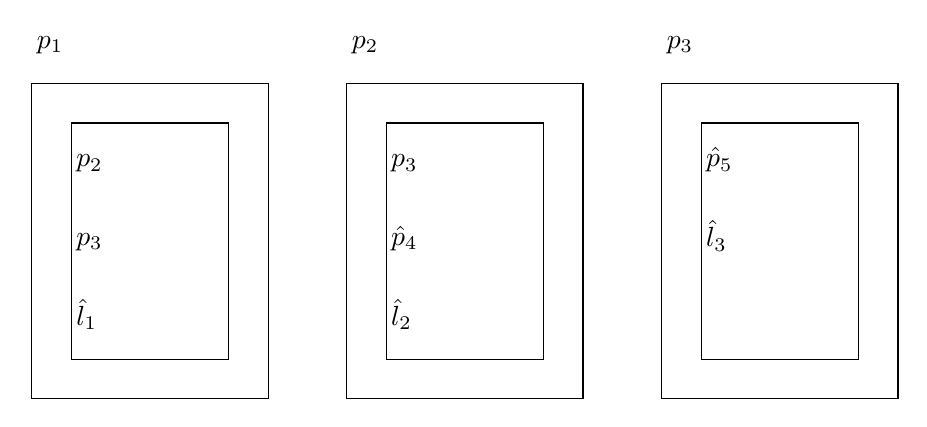
\begin{tikzpicture}
	\draw[draw=black, thin, solid] (-5.00,3.00) rectangle (-3.00,0.00);
	\draw[draw=black, thin, solid] (-1.50,3.50) rectangle (1.50,-0.50);
	\draw[draw=black, thin, solid] (2.50,3.50) rectangle (5.50,-0.50);
	\draw[draw=black, thin, solid] (-1.00,3.00) rectangle (1.00,0.00);
	\draw[draw=black, thin, solid] (3.00,3.00) rectangle (5.00,0.00);
	\draw[draw=black, thin, solid] (-5.50,3.50) rectangle (-2.50,-0.50);
	\node[black, anchor=south west] at (-5.56,3.75) {$p_1$};
	\node[black, anchor=south west] at (-1.56,3.75) {$p_2$};
	\node[black, anchor=south west] at (2.44,3.75) {$p_3$};
	\node[black, anchor=south west] at (-5.06,1.25) {$p_3$};
	\node[black, anchor=south west] at (-5.06,2.25) {$p_2$};
	\node[black, anchor=south west] at (-1.06,2.25) {$p_3$};
	\node[black, anchor=south west] at (-5.06,0.25) {$\hat l_1$};
	\node[black, anchor=south west] at (-1.06,0.25) {$\hat l_2$};
	\node[black, anchor=south west] at (2.94,1.25) {$\hat l_3$};
	\node[black, anchor=south west] at (-1.06,1.25) {$\hat p_4$};
	\node[black, anchor=south west] at (2.94,2.25) {$\hat p_5$};
\end{tikzpicture}
\caption{Przykład raportów o stanie techniki}
\label{fig:raport-ex}
\end{figure}

\subsubsection{Tworzenie grafu za pomocą danych z tabel
               raportów o stanie techniki}
\label{sec:graf-raporty}

Dane z raportów o stanie techniki tworzą graf skierowany
patentów $G$. Krawędź w takim grafie istnieje jeśli patent
$p_1$ zawiera w swoim raporcie wzmiankę o patencie~$p_2$.

Wracając do przykładu \cref{fig:raport-ex}, zastosowanie algorytmu 
tworzy graf o krawędziach $E = \{ (p_2, p_1), (p_3, p_1), (p_3, p_2) \}$ i
wierzchołkach $V = { p_1, p_2, p_3 }$.

\begin{figure}\centering
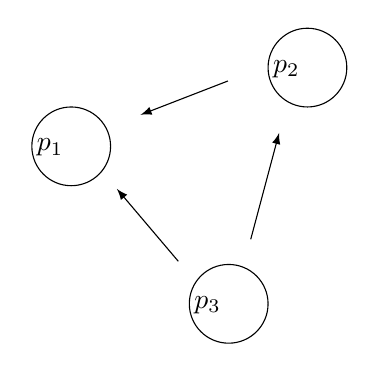
\begin{tikzpicture}
	\draw[draw=black, thin, solid] (-1.50,1.50) ellipse (0.50 and -0.50);
	\node[black, anchor=south west] at (-2.06,1.25) {$p_1$};
	\draw[draw=black, thin, solid] (1.50,2.50) ellipse (0.50 and -0.50);
	\draw[draw=black, thin, solid] (0.50,-0.50) ellipse (0.50 and -0.50);
	\node[black, anchor=south west] at (0.94,2.25) {$p_2$};
	\node[black, anchor=south west] at (-0.06,-0.75) {$p_3$};
	\draw[draw=black, -latex, thin, solid] (-0.14,0.04) -- (-0.92,0.96);
	\draw[draw=black, -latex, thin, solid] (0.78,0.32) -- (1.14,1.67);
	\draw[draw=black, -latex, thin, solid] (0.49,2.33) -- (-0.62,1.90);
\end{tikzpicture}
\caption{Graf dla przykładowego zestawu raportów \cref{fig:raport-ex}}
\label{fig:raport-ex-G}
\end{figure}

Zakładając, że wpisy ekspertów zawierają wyłącznie kody publikacji 
patentów, graf mógłby być stworzony przez bezpośrednie powiązanie
ich z danymi. Istotnym problemem w takiej sytuacji jest jakość \ac{OCR},
która jest dobra, ale nie pewna.
Wpisy ekspertów nie są jednak jednorodne w taki sposób. Problem
rozpoznania znaków nie jest jedyny, bo pojawiają się kolejne:

\begin{itemize}
\item wątpliwa jakość \ac{OCR}
\item wpisy to nie tylko kody patentowe
\item wspominane kody patentowe nie zawsze są publikacjami,
      mogą to być np. kody złożenia aplikacji
\end{itemize}

\begin{figure}[H]\centering
\includegraphics[width=0.8\textwidth]{ex-img/pat-ex-P.jpg}
\caption{Przykład odniesienia poprzez numer publikacji.}
\end{figure}

\begin{figure}[H]\centering
\includegraphics[width=0.8\textwidth]{ex-img/pat-ex-A.jpg}
\caption{Przykład odniesienia poprzez numer aplikacji.}
\end{figure}

\begin{figure}[H]\centering
\includegraphics[width=0.8\textwidth]{ex-img/pat-ex-A-P.jpg}
\caption{Przykład odniesienia poprzez numer aplikacji i publikacji
         jako jeden numer.}
\end{figure}

Sposobem na minimalizację zjawiska błędnych powiązań jest zastosowanie
algorytmu wyszukiwania (\cref{sec:wyszukiwanie}).

Ninejsze wyszukiwanie polega na wskazaniu sumy zbiorów
słów: numerów patentowych, słów języka naturalnego oraz dat. 
Wskazanie tej sumy zachodzi dla każdej pary wszystkich słów zapytań
ze wszystkimi słowami ze zbioru danych. Dodatkowo zachodzi łączenie
częściowe, które dopasowuje n-gramy poszczególnych słów. Od pewnego
minimalnego dopasowania zostają one uwzględnione. Całość wymaga
pewnych kroków optymalizacyjnych. Głównym jest zasada, że słowa
są dopasowywane tylko pod warunkiem, że zaszło dopasowanie numeru
patentu.

W trakcie wyszukiwania tworzona jest jego punktacja, aby odróżnić
wartościowe wyniki. Oprócz punktacji jest też ustalanie poziomu
wyszukiwania na podstawie tego jakie rzeczywiste dane są łącznikami.
Wybierane są wyłącznie pojedyncze, najlepsze wyniki.

Raporty \ac{PDF} nie posiadają adnotacji tekstowych. 
Znaczy to tyle, że dane są zawarte w sposób czytelny
jedynie dla człowieka i nie są dostępne dla urządzeń w sposób
ustruktoryzowany inny niż ciąg binarny pikseli.
Rozwiązaniem jest proces \ac{OCR}, który obrazy zawierające tekst
przekształca na kod binarny, które można przetwarzać na komputerze
jako ciągi znaków odpowiadające prawdziwemu tekstowi. Pierwszą
czynnością w tym procesie jest zastosowanie pakietu \textit{paddle}.
\todonote{Dodać link do \textit{paddle}}
\todonote{Opisać strukturę pat.}
Zastosowanie modułu pozwala na pozyskanie linijek tekstu z przypisaniem
do ich pozycji. Wynika z tego problem taki, że nie brak jest informacji
o tym gdzie zaczyna i kończy się tekst dotyczący wskazanej obserwacji.
W związku z tym nie sposób jest przypisać tekstu do odpowiednich
wpisów. Dodatkowo dochodzą problemy wynikające z błędów w procesie
skanowania samych dokumentów - zniekształcenia, zaciemnienia, czy
rotacje kartek sprawiają, że proces \ac{OCR} nie jest idealny.
Dodatkowo samo formatowanie nierzadko jest wadliwe co wynika
z wprowadzania danych jeszcze na etapie tworzenia dokumentów.



\subsubsection{Problemy standardowego \ac{OCR}}

\begin{enumerate}
\item data obs. 1. jest niżej niż linia tekstowa - 
nie wiadomo czy przypisać do obs. 1. czy do obs. 2.;
\item znak obs. 2. jest niżej niż powinien - nie wiadomo
czy przypisać do obs. 2. czy do obs. 3., a z tego wynika,
że nie wiadomo, czy obs. 2 w ogóle istnieje, czy jest też
rozwinięciem obs. 1;
\item zastrzeżenie obs. 3. jest bardzo blisko daty, a ta
z kolei to sam rok - nie wiadomo, czy zastrzeżenie jest częścią
daty.
\end{enumerate}

\begin{verbatim}
<NAGŁÓWEK ZNAKU>      <NAGŁÓWEK TEKSTU>                      <NAGŁ. ZAS.>
<ZNAK OBS=1>      <KOD PAT. OBS=1> <TEKST PAT. OBS=1><DATA OBS=1> <ZAS. OBS=1>
<ZNAK OBS=2>      <TEKST LITERATURY OBS=2>
                  <TEKST LITERATURY OBS=3>           <DATA OBS=3> <ZAS. OBS=3>
\end{verbatim}
\sidenote{Czy potrzeb. są przykł.?}
\todonote{Zrobić to jako obraz}

Problemy te są rozwiązywalne, ale zastosowanie zasad geometrii,
wykrywania linii oraz wyszukiwania słów kluczowych są niewystarczające
do osiągnięcia zadowalających wyników. Także sieci neuronowe oparte
o wskazane informacje nie radziły sobie z zadaniem.
\sidenote{Tzn. ja nie potrafi. zrobić takiej sieci}



\subsubsection{Zastosowanie dużego modelu językowego}

Do skutecznego pozyskania danych z dokumentów kluczowe było zastosowanie
dużych modeli językowych z multimodalnymi wejściami. Stan tej technologii
na dzień procesu wyciągania danych był na tyle zaawansowany, że
aspekty techniczne ograniczają się do zastosowania zewnętrznego \ac{API}
dla modelu \textit{openai} \textit{GPT4o}. Model ten w wystarczający
sposób był w stanie przetworzyć obrazy zawierające tekst na ustruktoryzowany
zbiór wpisów tekstowych.

Mimo, że model \textit{paddle} nie dawał wyników pozwalających na
poprawną dalszą analizę to pozwolił na ograniczenie kosztów. Znalezienie
słów kluczowych nagłówków i stopek tabeli z informacjami było wystarczające
aby przyciąć zdjęcia do obszarów zainteresowania.

\todonote{Opisać problem literówek}
\sidenote{Czy opisywać proces GPT4o?}


\bibliographystyle{plain}\bibliography{cit}

\listoffigures

\listoftables

\chapter*{Załączniki}
\begin{enumerate}
\item Płyta CD z niniejszą pracą w wersji elektronicznej.
\end{enumerate}

\chapter*{Streszczenie (Summary)}

\bigskip

\bigskip

\begin{center}
  \textbf{\tytul}
\end{center}

\bigskip

\begin{center}
  \textbf{\textit{\tytulangielski}}
\end{center}

\selecthyphenation{english}
{\it

}

\end{document}